\begin{columns}
  \begin{column}{0.4\textwidth}
    \centering

    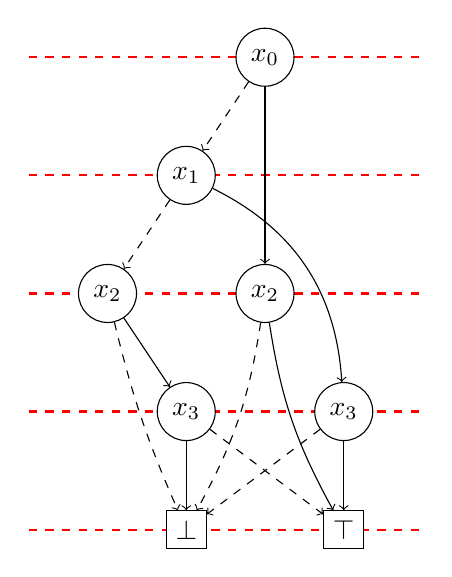
\begin{tikzpicture}
      % sweepline
      \onslide<2> { \draw[red, thick, dashed] (-3, 0)   -- ++(5, 0); }
      \onslide<3> { \draw[red, thick, dashed] (-3,-1.5) -- ++(5, 0); }
      \onslide<4> { \draw[red, thick, dashed] (-3,-3)   -- ++(5, 0); }
      \onslide<5> { \draw[red, thick, dashed] (-3,-4.5) -- ++(5, 0); }
      \onslide<6> { \draw[red, thick, dashed] (-3,-6)   -- ++(5, 0); }

      % nodes
      \node[shape=circle, draw=black, fill=white] at ( 0, 0)
      (0) {$x_0$};

      \node[shape=circle, draw=black, fill=white] at (-1,-1.5)
      (1) {$x_1$};

      \node[shape=circle, draw=black, fill=white] at (-2,-3)
      (21) {$x_2$};
      \node[shape=circle, draw=black, fill=white] at ( 0,-3)
      (22) {$x_2$};

      \node[shape=circle, draw=black, fill=white] at (-1,-4.5)
      (31) {$x_3$};
      \node[shape=circle, draw=black, fill=white] at ( 1,-4.5)
      (32) {$x_3$};

      % leafs
      \node[shape=rectangle, draw=black, fill=white] at (-1,-6)
      (bot) {$\bot$};
      \node[shape=rectangle, draw=black, fill=white] at ( 1,-6)
      (top) {$\top$};

      % arcs
      \draw[->, dashed]
        (0)  edge (1)
        (1)  edge (21)
        (21) edge[bend right=5] (bot)
        (22) edge[bend left=10] (bot)
        (31) edge (top)
        (32) edge (bot)
      ;

      \draw[->]
        (0)  edge (22)
        (1)  edge[bend left] (32)
        (21) edge (31)
        (22) edge[bend right=10] (top)
        (31) edge (bot)
        (32) edge (top)
      ;
    \end{tikzpicture}
  \end{column}
  \begin{column}{3em}
    \centering $\implies$
  \end{column}
  \begin{column}{0.4\textwidth}
    \centering

    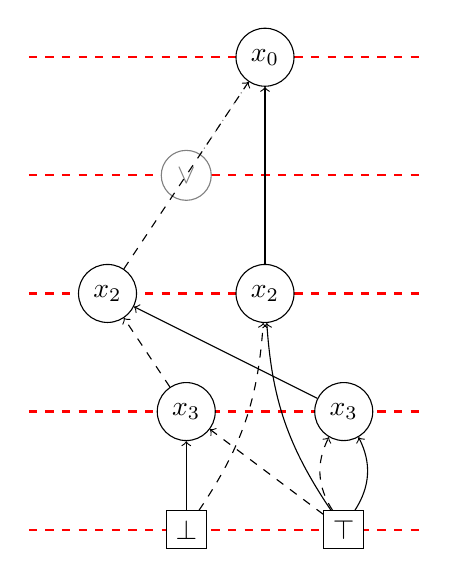
\begin{tikzpicture}
      % sweepline
      \onslide<2> { \draw[red, thick, dashed] (-3, 0)   -- ++(5, 0); }
      \onslide<3> { \draw[red, thick, dashed] (-3,-1.5) -- ++(5, 0); }
      \onslide<4> { \draw[red, thick, dashed] (-3,-3)   -- ++(5, 0); }
      \onslide<5> { \draw[red, thick, dashed] (-3,-4.5) -- ++(5, 0); }
      \onslide<6> { \draw[red, thick, dashed] (-3,-6)   -- ++(5, 0); }

      % levels
      \onslide<2-> {
        \node[shape=circle, draw=black, fill=white] at ( 0, 0)
        (0) {$x_0$};
      }

      \onslide<3> {
        \node[shape=circle, draw=gray, fill=white] at (-1,-1.5)
        (1) {\color{gray} $\lor$};

        \draw[-, dotted, gray] (1) edge (0);
      }

      \onslide<4-> {
        \node[shape=circle, draw=black, fill=white] at (-2,-3)
        (21) {$x_2$};
        \node[shape=circle, draw=black, fill=white] at ( 0,-3)
        (22) {$x_2$};

        \draw[->, dashed] (21) edge (0);
        \draw[->] (22) edge (0);
      }

      \onslide<5-> {
        \node[shape=circle, draw=black, fill=white] at (-1,-4.5)
        (31) {$x_3$};
        \node[shape=circle, draw=black, fill=white] at ( 1,-4.5)
        (32) {$x_3$};

        \draw[->, dashed]
          (31) edge (21)
        ;
        \draw[->]
          (32) edge (21)
        ;
      }

      \onslide<6-7> {
        \node[shape=rectangle, draw=black, fill=white] at (-1,-6)
        (bot) {$\bot$};
        \node[shape=rectangle, draw=black, fill=white] at ( 1,-6)
        (top) {$\top$};

        \draw[->, dashed]
          (bot) edge[bend right=15] (22)
          (top) edge (31)
          (top) edge[bend left] (32)
        ;
        \draw[->]
          (bot) edge (31)
          (top) edge[bend left=15] (22)
          (top) edge[bend right] (32)
        ;
      }
    \end{tikzpicture}
  \end{column}
\end{columns}